\documentclass{beamer}
\usepackage[english]{babel}
\usepackage[utf8]{inputenc}
\mode<presentation>{\usetheme{FS18}}
\usepackage{amsmath,amsthm, amssymb, latexsym}
\usepackage[orientation=portrait,size=a0,scale=1.4]{beamerposter}
\usepackage{natbib}
\bibliographystyle{unsrt}
\usepackage{subcaption}
\graphicspath{{../figures/graphics/}}
 
\title{Local Variance Optimization for the Autonomous Regulation of Echo State Networks}
\author{Fabian Schubert, Claudius Gros}
\institute{Institute for Theoretical Physics, Goethe University Frankfurt a.M.}
\date{Feb. 28th, 2019}

\renewcommand{\vec}[1]{\mathbf{#1}}

\newcommand{\vx}{\vec{x}}
\newcommand{\vy}{\vec{y}}
\newcommand{\vf}{\vec{f}}
\newcommand{\vsigm}{\boldsymbol{\sigma}}

\newcommand{\Err}{\mathrm{Err}}
\newcommand{\Exp}{\mathrm{E}}
\newcommand{\Var}{\mathrm{Var}}

\newcommand{\avgt}[1]{\left< #1 \right>_T}
\newcommand{\avgp}[1]{\left< #1 \right>_P}


\begin{document}
\begin{frame}[t]
\begin{columns}[t]
\begin{column}{.4\textwidth}
\begin{myblock}{Introduction}
Echo state networks have proven to be a powerful tool in the field of time series prediction~\citep{Jaeger_2001,Lukosevicius_2009}. Several approaches to the optimization of the dynamic reservoir have been investigated in the past, including global tuning for criticality~\cite{Livi_2016}, as well as local adaptation towards a given output distribution~\cite{Schrauwen_2008,Boedecker_2009}.

The spectral radius $|\Lambda_{\rm max}|$ of the synaptic weight matrix provides a measure to regulate the network in an appropriate working regime~\cite{Caluwaerts_2013}. We show that $|\Lambda_{\rm max}|$ can be regulated by local homeostasis of the variance $\sigma_y^2$ of neural activity. This variance control operates on the gain of the neural transfer function and its optimization target depends on the variance $\sigma_{\rm ext}^2$ of external input.

In contrast to previously proposed optimization rules via local intrinsic plasticity, our model relies on the assumption that external and recurrent input signals can be treated as two separate streams of information. The network can hence react autonomously to changes of the input statistics.
\end{myblock}

\begin{myblock}{Model Description}
\begin{align}
y_i^{t+1} &= \mathrm{tanh}\left( a_i^t I_i^{t+1} \right) \label{eq:reserv_dynamics}\\
I_i^{t+1} &= \sum_{j=1}^{N} W_{ij} y_j^t + E_i^{t+1} \label{eq:input_dynamics} \\
b_i^{t+1} &= b_i^t + \epsilon_{b} \left[ \avgt{y_i} - \mu_{t} \right] \\
a_i^{t+1} &= a_i^{t} + \epsilon_{a} \left[ \sigma_{t}^2 - \left( y_i^t - \overline{y}(t)_i\right)^2 \right] \label{eq:gain_dynamcis} \\
\overline{y}^{t+1}_i &= \epsilon_{\rm trail} \left[ y_i^{t+1} - \overline{y}^{t}_i\right]
\end{align}
By changing individual gain and bias values $a_i$ and $b_i$, the homeostatic control tries to drive the activity standard deviation and mean of every cell to the value given by $\sigma_{t}$ and $\mu_{t}$.
\end{myblock}

\begin{myblock}{Network Dynamics}
	\begin{figure}
		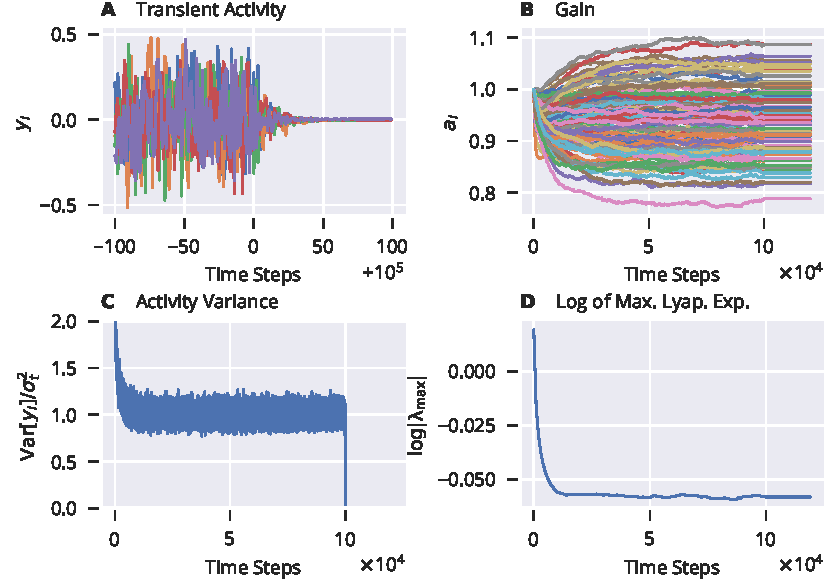
\includegraphics[width=\textwidth]{../figures/res_comp.pdf}
		\caption{Exemplary network dynamics, where the external input was switched off after $10^5$ time steps, followed by a transient period of decaying activity.}
		\label{fig:trans_dyn}
	\end{figure}
	\begin{itemize}
		\item By controlling the output variance of the neural activity, we can tune the network into a regime that exhibits subcritical, but transiently active dynamics in the absence of external input.
		\item This led to the question, how a homeostatic variance control could be used to tune network properties, even under changing input statistics. 
	\end{itemize}
\end{myblock}

\end{column}

\begin{column}{.5\textwidth}
\begin{myblock}{Changing Input and Target Variance}
	\begin{figure}
		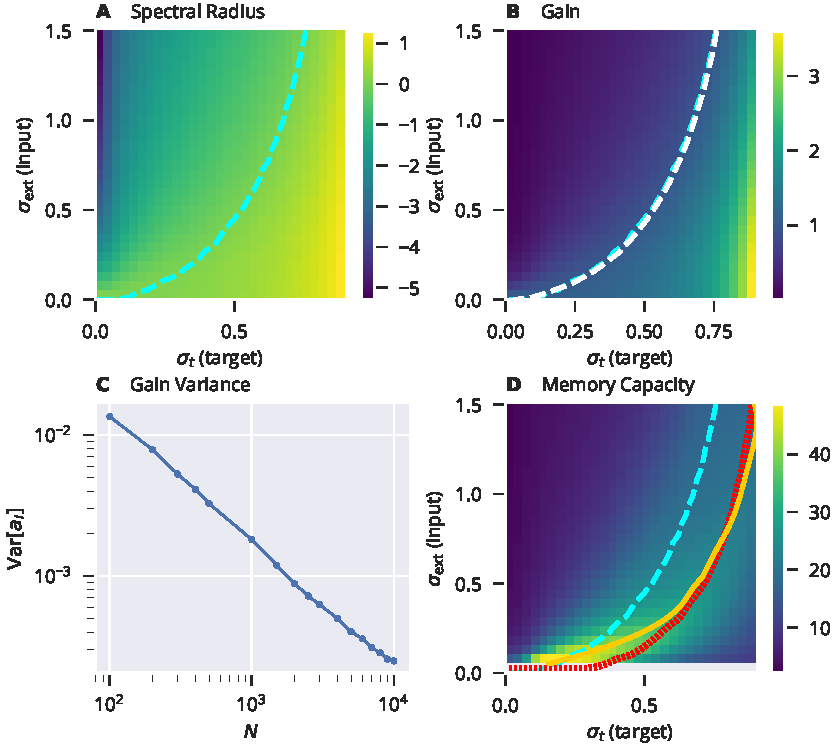
\includegraphics[width=\textwidth]{../figures/std_in_std_target_sweep_fig.pdf}
	\end{figure}
	
	\begin{figure}
		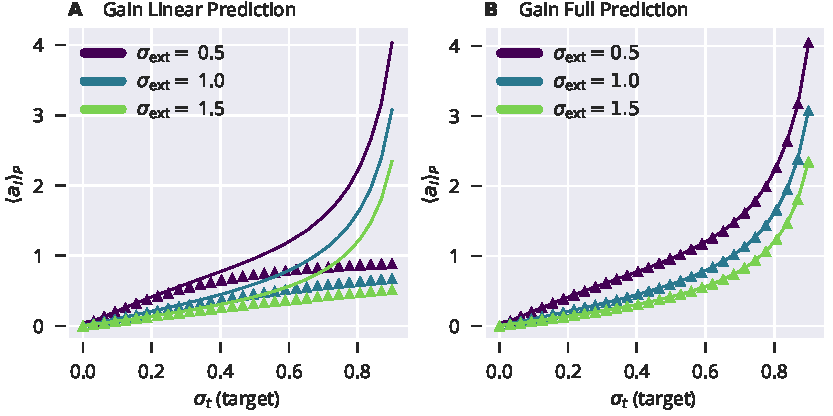
\includegraphics[width=\textwidth]{../figures/std_in_std_target_sweep_fig_cut.pdf}
	\end{figure}
\end{myblock}


\begin{myblock}{References}
	\bibliography{../../../../../lit_base.bib}
\end{myblock}

\end{column}
\end{columns}
\end{frame}
\end{document}
